\documentclass{beamer}
\usepackage[utf8]{inputenc}
\usepackage{graphicx}
\usepackage{amsmath,amssymb}
\usepackage{mathtools}
\usepackage{amsfonts}
\usepackage{stmaryrd}
\usepackage{amsthm}
\usepackage{algorithm}
\usepackage{algpseudocode}


\usepackage{stackengine}

\usepackage{subcaption}
\usepackage[T1]{fontenc}
\usepackage{libertine}
\usepackage[scaled=0.92]{inconsolata}
\usepackage[libertine]{newtxmath}
\usepackage{tikz}
\usetikzlibrary{bayesnet}
\usepackage{adjustbox}
\usepackage{multirow, multicol}
\usepackage{caption}
\usepackage{hyperref}

\usepackage{mwe}

\usetheme{Madrid}
\usecolortheme{default}
\setbeamertemplate{navigation symbols}{}


\newcommand{\cY}{\ensuremath{\mathcal{Y}}}
\newcommand{\cR}{\ensuremath{\mathcal{R}}}
\newcommand{\cX}{\ensuremath{\mathcal{X}}}
\renewcommand{\epsilon}{\varepsilon}
\renewcommand{\phi}{\varphi}
\newcommand{\floor}[1]{\left\lfloor #1 \right\rfloor}
\newcommand{\ceil}[1]{\left\lceil #1 \right\rceil}
\newcommand{\comb}[2]{\displaystyle{#2 \choose #1}}
\newcommand{\parts}{\mathcal{P}}
\newcommand{\permut}{\mathfrak{S}}
\newcommand{\id}{\text{Id}}
\newcommand{\indic}{\mathds{1}}
\renewcommand{\leq}{\leqslant}
\renewcommand{\geq}{\geqslant}
\newcommand{\mat}[2]{\mathcal{M}_{#1}(#2)}

\newcommand{\dd}{\text{d}}
\renewcommand{\vec}{\overrightarrow}
\renewcommand{\Im}{\mathfrak{Im}\ }
\newcommand{\Ker}{\text{Ker}\ }
\newcommand{\bijective}{%
  \hookrightarrow\mathrel{\mspace{-15mu}}\rightarrow
}
\newcommand{\surjective}{\twoheadrightarrow}
\newcommand{\injective}{\hookrightarrow}
\newcommand{\implication}{\Longrightarrow}
\newcommand{\reciprocal}{\Longleftarrow}
\newcommand{\equivalent}{\Longleftrightarrow}
\newcommand{\NN}{\ensuremath{\mathbb{N}}}
\newcommand{\RR}{\ensuremath{\mathbb{R}}}
\newcommand{\QQ}{\ensuremath{\mathbb{Q}}}
\newcommand{\ZZ}{\ensuremath{\mathbb{Z}}}
\newcommand{\CC}{\ensuremath{\mathbb{C}}}
\newcommand{\EE}{\ensuremath{\mathbb{E}}}
\newcommand{\PP}{\ensuremath{\mathbb{P}}}
\newcommand{\II}{\ensuremath{\mathds{1}}}
\newcommand{\IIp}[1]{\ensuremath{\mathds{1}\left\{ #1 \right\}}}
\newcommand{\cZ}{\ensuremath{\mathcal{Z}}}
\newcommand{\cN}{\ensuremath{\mathcal{N}}}
\newcommand{\cT}{\ensuremath{\mathcal{T}}}

\DeclareMathOperator{\mut}{mut}
\DeclareMathOperator{\stab}{Stab}
\DeclareMathOperator{\sg}{sg}
\DeclareMathOperator*{\argmax}{argmax}
\DeclareMathOperator*{\argmin}{argmin}
\renewcommand{\time}{\textsc{Time}}
\newcommand{\len}{\textsc{Length}}
\newcommand{\call}[1]{\textsc{#1}}
\newcommand{\bbrack}[1]{\left\llbracket#1\right\rrbracket}
\newcommand{\set}[1]{\ensuremath{\left\{ #1 \right\}}}

\DeclareMathOperator{\ucb}{UCB}

\author[]{Thomas \textsc{Michel}, Théo \textsc{Rudkiewicz} and Ali \textsc{Ramlaoui}}
\title[Clustering Multivariate Ordinal Data]{Clustering Multivariate Ordinal Data\\Alternative model and faster method}
\begin{document}

\frame{\titlepage}

\begin{frame}{Ordinal Data Clustering}
Found in :
\begin{itemize}
    \item Product review
    \item Health diagnostic (Evaluation of a patient's pain level)
    \item and others ... (Stage of growth of an organism in biology for instanceS)
\end{itemize}\\~\\

Why clustering:
\begin{itemize}
    \item Summarize large dataset
    \item Understand data
    \item Visualization
\end{itemize}
    
\end{frame}

\begin{frame}{Overview}
    \begin{itemize}
        \item Clustering multivariate ordinal data
              % \footnote{Study based on \textit{Christophe Biernacki and Julien Jacques. Model-based clustering of multivariate ordinal data relying on a stochastic binary search algorithm. Statistics and Computing, 26:929–943, 2016.}}
        \item Two univariate model: \begin{itemize}
                  \item Binary Ordinal Search (BOS)
                  \item Globally Ordered Data (GOD) $\star$
              \end{itemize}
        \item New fast parameter estimation method and open source implementation (\hyperlink{https://github.com/Thomick/Ordinal-data-clustering}{link}), maybe an online demonstration $\star$
        \item New experiments $\star$
    \end{itemize}

    \hfill\small $\star$ Our contribution
\end{frame}

\begin{frame}{Univariate probabilistic models: BOS}
    $n$ samples, $m$ categories
    \structure{BOS model}: Result of a binary search with noisy comparisons.

    \begin{figure}[htbp]
        \centering
        \begin{adjustbox}{width=0.8\textwidth}
            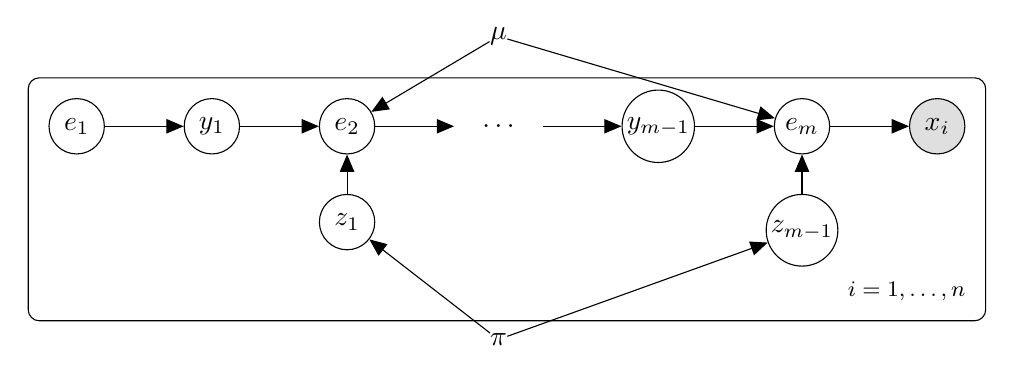
\begin{tikzpicture}
                \node[obs]                               (xi) {$x_i$};
                \node[latent, left=of xi]               (em) {$e_m$};
                \node[latent, below=of em, yshift=0.5cm]               (zm1) {$z_{m-1}$};
                \node[latent, left=of em]               (ym1) {$y_{m-1}$};
                \node[const, left=of ym1]               (dots) {$\quad\ldots\quad$};
                \node[latent, left=of dots]               (e2) {$e_2$};
                \node[latent, below=of e2, yshift=0.5cm]               (z1) {$z_1$};
                \node[latent, left=of e2]               (y1) {$y_1$};
                \node[latent, left=of y1]               (e1) {$e_1$};
                \node[const, above=of dots]    (mu) {$\mu$};
                \node[const, below=of dots, yshift=-1.6cm]  (pi) {$\pi$};

                \edge{e1}{y1};
                \edge{y1}{e2};
                \edge{z1}{e2};
                \edge{e2}{dots};
                \edge{dots}{ym1};
                \edge{ym1}{em};
                \edge{zm1}{em};
                \edge{em}{xi};
                \edge{mu}{e2};
                \edge{mu}{em};
                \edge{pi}{z1};
                \edge{pi}{zm1};

                \plate[inner sep=.25cm] {} {(xi)(e1)(zm1)(z1)} {$i=1, \ldots, n$};
            \end{tikzpicture}
        \end{adjustbox}
        \caption*{Graphical model of the stochastic Binary Ordinal Search.}
        \label{fig:graphical_model}
    \end{figure}
\end{frame}

\begin{frame}{Univariate probabilistic models : BOS}
    $n$ samples, $m$ categories
    \structure{BOS model}: Result of a binary search with noisy comparisons.

    \begin{example}
        With $m = 5, \mu = 2$:
        \begin{enumerate}
            \item $e_1 = \set{1, 2, 3, 4, 5} = \bbrack{1, m}$, $y_1 = 4$, $z_1 = 1$
            \item $e_2 = \set{1, 2, 3}, y_2 = 2, z_2 = 0$
            \item $e_3 = \set{1}, y_3 = 1, z_3 = 0$
            \item $e_4 = \set{1}, y_4 = 1, z_4 = 1$
            \item $e_5 = \set{1}$
        \end{enumerate}
    \end{example}
\end{frame}

\begin{frame}{Parameter estimation}
    \begin{block}{Maximum likelihood estimation}
        We have a set of $n$ independent observations $X = (x_i)_{i \in [n]}$, where $x_i \in \bbrack{1, m}$ follow a distribution $P$ with parameters $\mu, \pi$ with $\mu \in \bbrack{1, m}$

        The goal of MLE is:
        $$(\mu, \pi) = \argmax_{(\mu, \pi) \in \bbrack{1, m} \times [0, 1]} \Pr(X | \mu, \pi)$$

        (or equivalently 
        $$(\mu, \pi) = \argmax_{(\mu, \pi) \in \bbrack{1, m} \times [0, 1]} \log \Pr(X | \mu, \pi)$$
    \end{block}
\end{frame}

\begin{frame}{Likelihoods}
\begin{figure}
    \centering
    \includegraphics[width=0.9\textwidth]{Attachments/log_likelihoods_bos.png}
    \caption{Log-likelihoods for each possible $\mu$ for $n = 100$ samples with the true parameters being $m = 5$, $\mu=2$ and $\pi = 0.4$ }
    \label{fig:log_likelihoods}
\end{figure}
\end{frame}

\begin{frame}{Ternary search algorithm}
    \begin{theorem}
        $L_X(\mu, \bullet) : \pi \mapsto \log P(X | \mu, \pi)$ is strictly concave.
    \end{theorem}

    \pause
    
    \begin{block}{Ternary search}
        $L_X(\mu, \bullet)$ can be maximized at precision $\epsilon$ with ternary search in $\Theta(\ln \frac{1}{\epsilon})$ evaluation.
    \end{block}    
\end{frame}


\begin{frame}{Likelihood estimation}
\begin{theorem}
    We can efficiently compute $\Pr(x | \mu, \bullet)$ as it is a polynomial function of degree $m$.
\end{theorem}
\begin{proof}    
    \begin{align}
    \Pr(x | x \in e_j, \mu, \pi) 
    &= \sum_{e_{j+1} \subset e_j} \Pr(x, e_{j+1} | x \in e_j, \mu, \pi) \\
    &= \sum_{e_{j+1} \subset e_j} \Pr(x | e_{j+1}, x \in e_j, \mu, \pi) \Pr(e_{j+1} | e_j, \mu, \pi) \\
    &= \sum_{e_{j+1} \subset e_j ; x\in e_{j+1}} \Pr(x | x \in e_{j+1}, \mu, \pi) \Pr(e_{j+1} | e_j, \mu, \pi)
    \end{align}
\end{proof}
\end{frame}

\begin{frame}{MLE complexity}

\begin{block}{Complexity}
    \begin{itemize}
        \item Pre-compute the $m^3$ coefficients of the polynomials is done through dynamic programming in $\Theta(m^5)$
        \item Group the data by value is done in $\Theta(n)$ (\textit{ie} $(1, 1, 2, 4)$ to $(1:2, 2:1, 3:0, 4:1)$
        \item MLE optimization in $\Theta(m^3 \ln\frac{1}{\epsilon})$ : one optimization per $\mu$, each optimization is $\Theta(\ln{1}{\epsilon})$ evaluation, each evaluation is $\Theta(m^2)$ ($m$ evaluation of polynomial of degree $m$)
    \end{itemize}
\end{block}

\end{frame}

\begin{frame}{Univariate probabilistic models}
        \structure{GOD model}: Most probable result of a linear search with noisy comparisons.
        
        \begin{figure}[htbp]
        \centering
        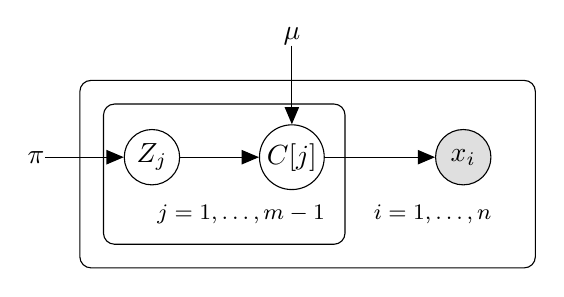
\begin{tikzpicture}
            \node[obs]                               (xj) {$x_i$};
            \node[latent, left=1.4cm of xj]               (cj) {$C[j]$};
            \node[latent, left=of cj]               (zj) {$Z_j$};
            \node[const, left=of zj]    (pi) {$\pi$};
            \node[const, above=of cj]  (mu) {$\mu$};

            \edge{zj}{cj};
            \edge{cj}{xj};
            \edge {mu} {cj};
            \edge {pi} {zj};

            \plate[inner sep=.55cm] {}{(xj)(cj)(zj)}{$i=1, \ldots, n$};
            \plate[inner sep=.25cm] {}{(cj)(zj)}{$j=1, \ldots, m-1$};
        \end{tikzpicture}
        \caption*{Graphical model of the GOD model.}
        \label{fig:god_graphical_model}
    \end{figure}
\end{frame}


\begin{frame}{Univariate probabilistic models : GOD}

    \begin{example}
        With $m = 5, \mu = 2$:
        \begin{itemize}
            \item $Z = (\top, \top, \top, \bot)$

            \item $C = (\mu \geq 1, \mu \geq 2, \mu < 3, \mu \geq 4)$

            \item $E = (2, 1, 2, 1)$

            \item $x = 2$
        \end{itemize}
    \end{example}
\end{frame}


\begin{frame}{Parameter estimation}
    \begin{definition}
    We define for $x \in \bbrack{1, m}$,:
\[ \mathcal{C}_x := \set{c \in \set{0, 1}^{m-1} | x \in \argmin_{k \in \bbrack{1, m}} \norm{c - E_k}_1 }\]
\end{definition}

\begin{definition}
    We define for $x \in \bbrack{1, m}, \mu \in \bbrack{1, m}, d \in \bbrack{0, m-1}$:
    \[ u(\mu, x, d) := \sum_{c \in \mathcal{C}_x / \norm{c - E_{\mu}}_1 = d}  \card{\argmin_{k \in \bbrack{1, m}} \norm{c - E_k}_1}^{-1}\]
\end{definition}

\end{frame}

\begin{frame}{Likelihood}
    \begin{theorem}{Observation likelihood}
    \label{thm:p_x_knowing_pi_mu}
    \[\Pr(x | \pi, \mu) = \pi^{m-1} \sum_{d = 0}^{m-1} \left(\frac{1 - \pi}{\pi}\right)^d u(x, \mu, d)\]
\end{theorem}


\begin{block}{Complexity }
    
    $O(m2^m)$ precomputation
    
    $\Theta(m^3 \log \frac{1}{\epsilon} + n)$
\end{block}

\end{frame}
\begin{frame}{AECM algorithm}
    Alternating Expectation-Conditional Maximization (AECM) algorithm allows finding cluster in data where each cluster is created by the same univariate probabilistic model.

    \scalebox{0.8}{
\begin{minipage}{1.2\textwidth}
\begin{algorithm}[H]
\caption{AECM}
\label{alg:aecm}
\begin{algorithmic}[1]
\Require Number of clusters $K$
\While {log-likelihood increase}
    \State \textbf{E Step}: For each sample, compute the conditional probability of belonging to each cluster given the current estimation of the model parameters, ie.
    $$\text{For $i\in\{1,...,n\}$ and $k\in\{1,...,K\}$, compute }p(i\in C_k | x_i, \boldsymbol{\alpha}, \boldsymbol{\mu}, \boldsymbol{\pi})$$
    \State \textbf{M Step}: Update the estimation of the model parameters using the probabilities of the previous step.
    \State \quad - Mixing proportion $\boldsymbol{\alpha}$
    \State \quad - Component parameters $(\mu_k,\pi_k)_{i=k}^K$ using the parameter estimation algorithm of the BOS or GOD models
\EndWhile
\end{algorithmic}
\end{algorithm}
\end{minipage}
}
\end{frame}

\begin{frame}{Experiments}
    \begin{itemize}
        \item We compare the runtime of our implementation of the BOS model with the original R package (\textit{ordinalClust}) provided by the authors of the paper.
            %\cite{selosse2021ordinalclust}.
    \end{itemize}

    \begin{columns}

    \column{0.5\textwidth}
    \begin{figure}[htpb]
        \centering
        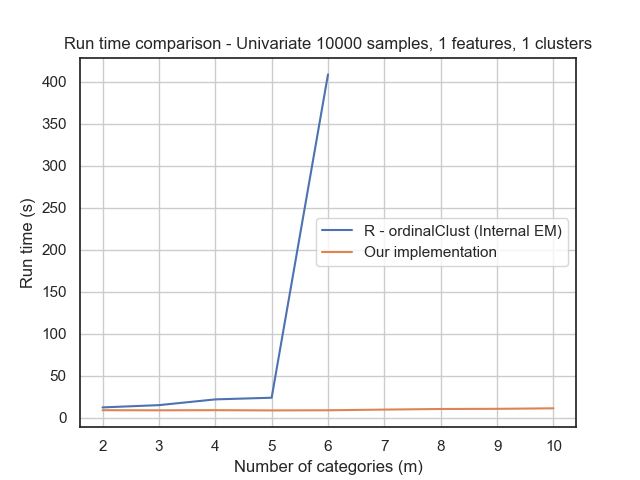
\includegraphics[width=0.8\textwidth]{python_figures/run_time_comparison_univariate.png}
        \caption*{Univariate model}
        \label{fig:runtimes_univariate}
    \end{figure}

    \column{0.5\textwidth}
    \begin{figure}[htpb]
        \centering
        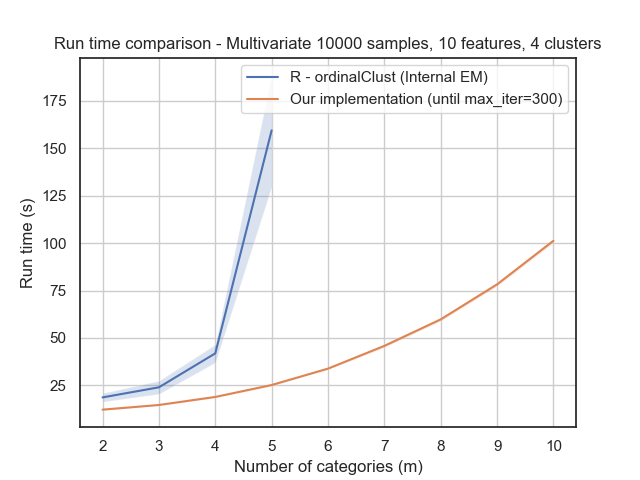
\includegraphics[width=0.8\textwidth]{python_figures/run_time_comparison_multivariate.png}
        \caption*{Multivariate model}
        \label{fig:runtimes_multivariate}
    \end{figure}
        
    \end{columns}

    \begin{itemize}
        \item The original implementation is exponential in the number of categories, while our implementation is polynomial.
    \end{itemize}

\end{frame}

\begin{frame}{Experiments}
    \begin{itemize}
        \item Test of the AECM estimation for both models on generated datasets from the corresponding distributions.
        \item Different parameters are tested and the runtimes, the average of the $L_1$ distances between the true and estimated parameters after applying optimal transport to find the correct clusters, are reported (10 runs). 
    \end{itemize}

    \begin{table}[H]
        \centering
        \begin{minipage}{.48\columnwidth}
            \centering
            \begin{adjustbox}{width=\columnwidth}
                \begin{tabular}{lllllrrrr}
                 &  &  &  &  & Runtime (s) & $\Delta \alpha$ & $\Delta \mu$ & $\Delta \pi$ \\
                Init. & $n$ & $n_{clusters}$ & $d$ & $n_{cats}$ &  &  &  &  \\
                \cline{1-9} \cline{2-9} \cline{3-9} \cline{4-9}
                \multirow[t]{16}{*}{random} & \multirow[t]{8}{*}{50} & \multirow[t]{4}{*}{3} & \multirow[t]{2}{*}{3} & 2 & 0.026 & 0.122 & 0.200 & 0.161 \\
                 &  &  &  & 3 & 0.055 & 0.117 & 0.167 & 0.116 \\
                \cline{4-9}
                 &  &  & \multirow[t]{2}{*}{5} & 2 & 0.053 & 0.056 & 0.130 & 0.094 \\
                 &  &  &  & 3 & 0.064 & 0.037 & 0.133 & 0.050 \\
                \cline{3-9} \cline{4-9}
                 &  & \multirow[t]{4}{*}{5} & \multirow[t]{2}{*}{3} & 2 & 0.061 & 0.118 & 0.283 & 0.234 \\
                 &  &  &  & 3 & 0.160 & 0.140 & 0.489 & 0.195 \\
                \cline{4-9}
                 &  &  & \multirow[t]{2}{*}{5} & 2 & 0.127 & 0.087 & 0.260 & 0.192 \\
                 &  &  &  & 3 & 0.235 & 0.051 & 0.160 & 0.114 \\
                \cline{2-9} \cline{3-9} \cline{4-9}
                 & \multirow[t]{8}{*}{250} & \multirow[t]{4}{*}{3} & \multirow[t]{2}{*}{3} & 2 & 0.084 & 0.143 & 0.150 & 0.082 \\
                 &  &  &  & 3 & 0.059 & 0.066 & 0.067 & 0.049 \\
                \cline{4-9}
                 &  &  & \multirow[t]{2}{*}{5} & 2 & 0.085 & 0.049 & 0.040 & 0.052 \\
                 &  &  &  & 3 & 0.135 & 0.025 & 0.093 & 0.026 \\
                \cline{3-9} \cline{4-9}
                 &  & \multirow[t]{4}{*}{5} & \multirow[t]{2}{*}{3} & 2 & 0.074 & 0.109 & 0.150 & 0.153 \\
                 &  &  &  & 3 & 0.111 & 0.093 & 0.156 & 0.104 \\
                \cline{4-9}
                 &  &  & \multirow[t]{2}{*}{5} & 2 & 0.207 & 0.060 & 0.120 & 0.114 \\
                 &  &  &  & 3 & 0.336 & 0.035 & 0.093 & 0.057 \\
                \cline{1-9} \cline{2-9} \cline{3-9} \cline{4-9}
                \end{tabular}
            \end{adjustbox}
            % \caption{Results of the experiments for the AECM algorithm no synthetic data with the BOS distribution. The parameters are the number of samples $n$, the number of clusters $n_{clusters}$, the dimension $d$ and the number of categories $n_{cats}$. The deltas are the average of the $L_1$ distances between the true and estimated parameters after applying optimal transport to find the correct clusters.}
            \caption*{AECM for BOS model.}
            \label{tab:results_bos}
        \end{minipage} \hspace{.02\columnwidth}%
        \begin{minipage}{.48\columnwidth}
            \centering
            \begin{adjustbox}{width=\columnwidth}
                \begin{tabular}{lllllrrrr}
                 &  &  &  &  & Runtime (s) & $\Delta \alpha$ & $\Delta \mu$ & $\Delta \pi$ \\
                Init. & $n$ & $n_{clusters}$ & $d$ & $n_{cats}$ &  &  &  &  \\
                \cline{1-9} \cline{2-9} \cline{3-9} \cline{4-9}
                \multirow[t]{16}{*}{random} & \multirow[t]{8}{*}{50} & \multirow[t]{4}{*}{3} & \multirow[t]{2}{*}{3} & 2 & 0.023 & 0.155 & 0.367 & 0.109 \\
                 &  &  &  & 3 & 0.047 & 0.152 & 0.367 & 0.063 \\
                \cline{4-9}
                 &  &  & \multirow[t]{2}{*}{5} & 2 & 0.038 & 0.073 & 0.130 & 0.057 \\
                 &  &  &  & 3 & 0.077 & 0.088 & 0.147 & 0.032 \\
                \cline{3-9} \cline{4-9}
                 &  & \multirow[t]{4}{*}{5} & \multirow[t]{2}{*}{3} & 2 & 0.035 & 0.149 & 0.533 & 0.157 \\
                 &  &  &  & 3 & 0.077 & 0.172 & 0.567 & 0.114 \\
                \cline{4-9}
                 &  &  & \multirow[t]{2}{*}{5} & 2 & 0.061 & 0.106 & 0.410 & 0.117 \\
                 &  &  &  & 3 & 0.126 & 0.131 & 0.380 & 0.075 \\
                \cline{2-9} \cline{3-9} \cline{4-9}
                 & \multirow[t]{8}{*}{250} & \multirow[t]{4}{*}{3} & \multirow[t]{2}{*}{3} & 2 & 0.031 & 0.152 & 0.283 & 0.104 \\
                 &  &  &  & 3 & 0.055 & 0.149 & 0.300 & 0.055 \\
                \cline{4-9}
                 &  &  & \multirow[t]{2}{*}{5} & 2 & 0.045 & 0.072 & 0.140 & 0.052 \\
                 &  &  &  & 3 & 0.084 & 0.080 & 0.153 & 0.027 \\
                \cline{3-9} \cline{4-9}
                 &  & \multirow[t]{4}{*}{5} & \multirow[t]{2}{*}{3} & 2 & 0.044 & 0.144 & 0.517 & 0.148 \\
                 &  &  &  & 3 & 0.085 & 0.150 & 0.522 & 0.109 \\
                \cline{4-9}
                 &  &  & \multirow[t]{2}{*}{5} & 2 & 0.069 & 0.119 & 0.390 & 0.105 \\
                 &  &  &  & 3 & 0.134 & 0.085 & 0.313 & 0.054 \\
                \cline{1-9} \cline{2-9} \cline{3-9} \cline{4-9}
                \end{tabular}
            \end{adjustbox}
            % \caption{Results of the experiments for the AECM algorithm no synthetic data with the GOD model. The parameters are the number of samples $n$, the number of clusters $n_{clusters}$, the dimension $d$ and the number of categories $n_{cats}$. The deltas are the average of the $L_1$ distances between the true and estimated parameters after applying optimal transport to find the correct clusters.}
            \caption*{AECM for GOD model.}
            \label{tab:results_god}
        \end{minipage}
    \end{table}
\end{frame}

\begin{frame}{Experiments}
    \only<1>{
    \vspace{-1.5cm}
    \begin{itemize}
        \item We also try to visualize the clusters found by the AECM algorithm on the synthetic datasets.
        \item Data type is ordinal $\Rightarrow$ We use t-SNE to visualize the clusters in a 2D continuous space.
    \end{itemize}
    }

    \only<2>{
    \begin{figure}[htpb]
        \centering
        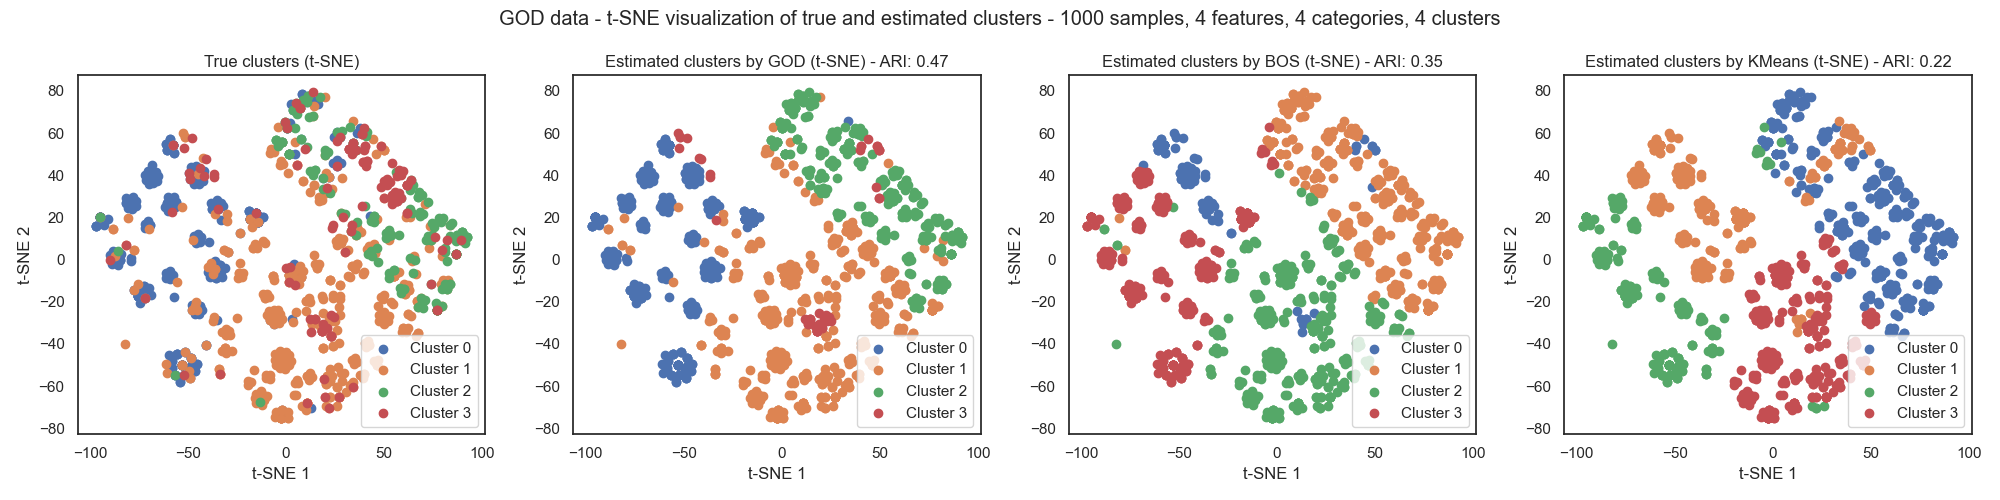
\includegraphics[width=1\textwidth]{python_figures/tsne_god_n1000_d4_m4_k4.png}
        \caption*{}
        \label{fig:tsne_god_n1000_d4_m4_k4}
    \end{figure}

    \vspace{-1.5cm}

    \begin{figure}[htpb]
        \centering
        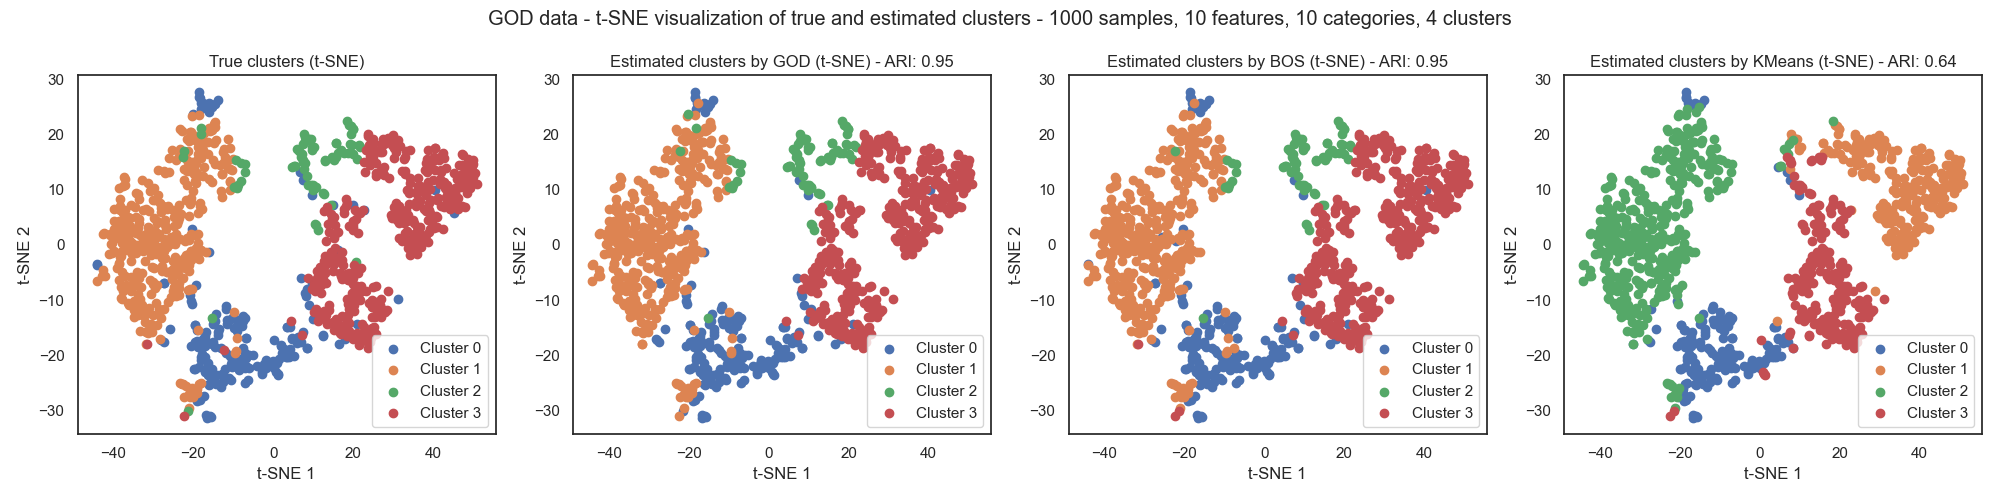
\includegraphics[width=1\textwidth]{python_figures/tsne_god_n1000_d10_m10_k4.png}
        \caption*{}
        \label{fig:tsne_god_n1000_d10_m10_k4}
    \end{figure}
}

\end{frame}

\begin{frame}{Experiments}

    \only<1>{
        \footnotesize{
        The adjusted Rand index (ARI) is a measure of the similarity between two clusterings. It is defined as follows:
        \begin{equation*}
            ARI = \frac{\sum_{ij} \binom{n_{ij}}{2} - \left[\sum_i \binom{a_i}{2} \sum_j \binom{b_j}{2}\right] / \binom{n}{2}}{\frac{1}{2}\left[\sum_i \binom{a_i}{2} + \sum_j \binom{b_j}{2}\right] - \left[\sum_i \binom{a_i}{2} \sum_j \binom{b_j}{2}\right] / \binom{n}{2}}
        \end{equation*}
        \begin{itemize}
            \item $n_{ij}$ number of pairs of elements in the same cluster in the first partition the second partition,
            \item $a_i$ number of pairs of elements in the same cluster in the first partition,
            \item $b_j$ number of pairs of elements in the same cluster in the second partition.
            \item The ARI is a number between -0.5 (discordant clusterings) and 1 (perfectly concordant clusterings, up to a permutation).
        \end{itemize}
        }
    }

    \only<2>{
    \begin{itemize}
        \item Synthetic data is generated from different models.
        \item We compare the ARI of the clusters found by different clustering methods for every model.
        \item Shows the ability of the AECM algorithm to find the correct clusters from different distributions.
    \end{itemize}

    \begin{table}[H]
        \begin{minipage}{.48\columnwidth}
        \begin{adjustbox}{width=\columnwidth}
        \begin{tabular}{lllllrrrr}
         &  &  &  &  & ARI BOS & ARI GOD & ARI KMeans & ARI GMM \\
        Data model & n & k & d & m &  &  &  &  \\
        \cline{1-9}
        \multirow[t]{3}{*}{BOS} & \multirow[t]{3}{*}{10000} & \multirow[t]{3}{*}{4} & 4 & 4 & 0.389 & 0.367 & 0.189 & 0.192 \\
        \cline{4-9}
         &  &  & 7 & 7 & 0.855 & 0.840 & 0.395 & 0.450 \\
        \cline{4-9}
         &  &  & 10 & 10 & 0.972 & 0.963 & 0.691 & 0.580 \\
        \end{tabular}
        \end{adjustbox}
        \end{minipage} \hspace{.02\columnwidth}%
        \begin{minipage}{.48\columnwidth}
        \begin{adjustbox}{width=\columnwidth}
        \begin{tabular}{lllllrrrr}
         &  &  &  &  & ARI BOS & ARI GOD & ARI KMeans & ARI GMM \\
        Data model & n & k & d & m &  &  &  &  \\
        \cline{1-9}
        \multirow[t]{3}{*}{GOD} & \multirow[t]{3}{*}{10000} & \multirow[t]{3}{*}{4} & 4 & 4 & 0.260 & 0.494 & 0.308 & 0.308 \\
        \cline{4-9}
         &  &  & 7 & 7 & 0.548 & 0.828 & 0.481 & 0.499 \\
        \cline{4-9}
         &  &  & 10 & 10 & 0.707 & 0.829 & 0.649 & 0.614 \\
        \end{tabular}
        \end{adjustbox}
        \end{minipage}
        \begin{minipage}{.48\columnwidth}
        \begin{adjustbox}{width=\columnwidth}
        \begin{tabular}{lllllrrrr}
         &  &  &  &  & ARI BOS & ARI GOD & ARI KMeans & ARI GMM \\
        Data model & n & k & d & m &  &  &  &  \\
        \cline{1-9}
        \multirow[t]{3}{*}{Blobs} & \multirow[t]{3}{*}{10000} & \multirow[t]{3}{*}{4} & 4 & 4 & 0.747 & 0.928 & 0.988 & 0.988 \\
        \cline{4-9}
         &  &  & 7 & 7 & 0.719 & 0.875 & 0.993 & 0.993 \\
        \cline{4-9}
         &  &  & 10 & 10 & 0.976 & 0.246 & 1.000 & 1.000 \\
        \end{tabular}
        \end{adjustbox}
        \end{minipage}
        \begin{minipage}{.48\columnwidth}
        \begin{adjustbox}{width=\columnwidth}
        \begin{tabular}{lllllrrrr}
         &  &  &  &  & ARI BOS & ARI GOD & ARI KMeans & ARI GMM \\
        Data model & n & k & d & m &  &  &  &  \\
        \cline{1-9}
        \multirow[t]{3}{*}{GMM} & \multirow[t]{3}{*}{10000} & \multirow[t]{3}{*}{4} & 4 & 4 & 0.000 & -0.000 & -0.000 & -0.000 \\
        \cline{4-9}
         &  &  & 7 & 7 & 0.000 & -0.001 & 0.001 & 0.001 \\
        \cline{4-9}
         &  &  & 10 & 10 & 0.000 & 0.000 & 0.003 & 0.002 \\
        \end{tabular}
        \end{adjustbox}
        \end{minipage}
    \end{table}
    }


    
\end{frame}

\begin{frame}{Experiments}

    \begin{itemize}
        \footnotesize
        \item Application of the clustering methods on real-life ordinal datasets.
        \item The classification score are reported according to a natural ordering of the categories (ie. in real life, they might not necessarily be ordered numerically).
    \end{itemize}

    \begin{table}
    \tiny
    \adjustbox{max width=0.7\textwidth}{
    \begin{tabular}{llllll}
     &  & \textbf{(s)} & \textbf{F1} & \textbf{Acc.} & \textbf{ARI} \\
    Dataset & Method &  &  &   &  \\
    \multirow[t]{6}{*}{\textbf{Zoo}} & \textbf{BOS Random} & 0.86 & 0.89 & 0.89 & 0.85 \\
    \textbf{} & \textbf{BOS K-Means} & 0.35 & 0.81 & 0.80 & 0.83 \\
    \textbf{} & \textbf{GOD Random} & 0.65 & 0.90 & 0.90 & 0.91 \\
    \textbf{} & \textbf{GOD K-Means} & 0.25 & 0.81 & 0.80 & 0.83 \\
    \textbf{} & \textbf{K-Means} & 0.01 & 0.84 & 0.85 & 0.83 \\
    \textbf{} & \textbf{Gaussian} & 2.58 & 0.77 & 0.74 & 0.66 \\
    \cline{1-6}
    \multirow[t]{6}{*}{\textbf{Car Evaluation}} & \textbf{BOS Random} & 0.20 & 0.46 & 0.38 & 0.01 \\
    \textbf{} & \textbf{BOS K-Means} & 0.57 & 0.45 & 0.38 & 0.04 \\
    \textbf{} & \textbf{GOD Random} & 0.19 & 0.48 & 0.42 & -0.00 \\
    \textbf{} & \textbf{GOD K-Means} & 0.54 & 0.39 & 0.31 & -0.00 \\
    \textbf{} & \textbf{K-Means} & 0.01 & 0.35 & 0.29 & 0.00 \\
    \textbf{} & \textbf{Gaussian} & 0.05 & 0.41 & 0.33 & 0.01 \\
    \cline{1-6}
    \multirow[t]{6}{*}{\textbf{Hayes-Roth}} & \textbf{BOS Random} & 0.08 & 0.45 & 0.46 & 0.02 \\
    \textbf{} & \textbf{BOS K-Means} & 0.08 & 0.34 & 0.33 & -0.01 \\
    \textbf{} & \textbf{GOD Random} & 0.28 & 0.40 & 0.41 & 0.01 \\
    \textbf{} & \textbf{GOD K-Means} & 0.06 & 0.36 & 0.36 & -0.01 \\
    \textbf{} & \textbf{K-Means} & 0.01 & 0.34 & 0.33 & -0.01 \\
    \textbf{} & \textbf{Gaussian} & 0.03 & 0.45 & 0.45 & 0.07 \\
    \cline{1-6}
    \multirow[t]{6}{*}{\textbf{Caesarian}} & \textbf{BOS Random} & 0.09 & 0.53 & 0.53 & -0.01 \\
    \textbf{} & \textbf{BOS K-Means} & 0.02 & 0.53 & 0.53 & -0.01 \\
    \textbf{} & \textbf{GOD Random} & 0.10 & 0.53 & 0.53 & -0.01 \\
    \textbf{} & \textbf{GOD K-Means} & 0.07 & 0.53 & 0.53 & -0.01 \\
    \textbf{} & \textbf{K-Means} & 0.01 & 0.56 & 0.56 & 0.00 \\
    \textbf{} & \textbf{Gaussian} & 0.01 & 0.60 & 0.60 & 0.03 \\
    \cline{1-6}
    \end{tabular}
    }
    \end{table}

\end{frame}

\begin{frame}{Demonstration}
    \href{https://ipolcore.ipol.im/demo/clientApp/demo.html?id=77777000487}{Open Demo}
    \begin{figure}
        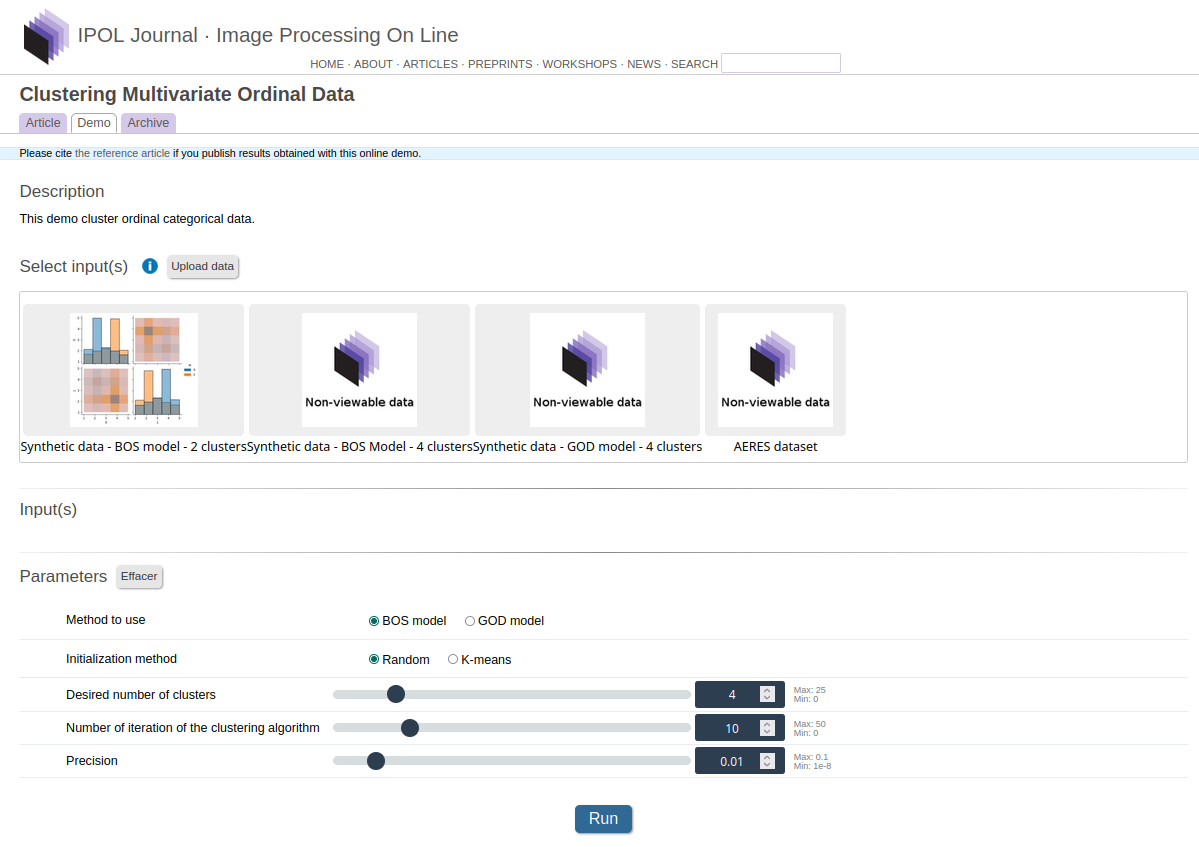
\includegraphics[width=0.8\textwidth]{Attachments/demo.png}
    \end{figure}
\end{frame}

\end{document}
